\section{Driver Interface Module}

The driver interface module implements the design specified in Sec.\ \ref{sec:Driver-Interface-Module}. The hardware and software are discussed in this section. Figure \ref{fig:driver_interface_pcb} shows a photo of the completely populated and debugged driver interface module PCB.

\begin{figure}[h]
\centering
\includegraphics[scale=1]{implementation/figures/driver_interface_pcb.eps}
\caption{Photograph of the populated driver interface module PCB.}\label{fig:driver_interface_pcb}
\end{figure}

\subsection{Hardware}

The driver interface module provides all of the support hardware needed for the LCD module to function. An \emph{FPC} connector, \emph{LCD bias boost converter}, \unit{+3.3}{\volt} power supply, latch, and level translators are all included in the module. Additionally, three rotary encoders are soldered onto the board. Connectors are soldered onto the back of the PCB to connect the steering wheel-mounted push buttons and paddles.

\subsubsection{LCD Module}

The LCD module used in the driver interface implementation is a pre-packaged LCD module from Newhaven Display. Along with the actual LCD panel, a built-in display controller chip and display RAM are included. Interfacing with the LCD module entails interfacing with it's controller chip, a SED1335 LCD controller IC from Seiko Epson Corporation. The controller chip handles all of the low level functionality of the LCD, such as generating pixel clocks and drawing to the screen from the LCD RAM. It also provides a character generator.

\subsubsection{LCD Bias Circuit}

The LCD screen requires a large bias voltage of \unit{+22}{\volt} to operate \cite{LCD_Module}. A Linear Technology LT1615 step-up DC/DC converter is used as the heart of a boost converter circuit to generate this bias voltage. The circuit schematic for the boost converter is shown in Fig.\ \ref{fig:lcd_boost_converter}.

\begin{figure}[htp]
 \centering
 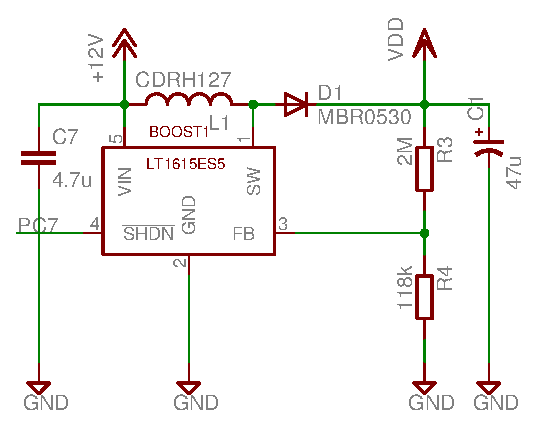
\includegraphics[scale=0.8]{implementation/figures/driver_interface_lcd_bias_circuit.eps}
 \caption{Schematic of the LCD boost converter circuit.}
 \label{fig:lcd_boost_converter}
\end{figure}

The data-sheet provides formulas for calculating the value of the inductor $L_1$. We calculated an inductor value of \unit{10}{\micro\henry}, which worked perfectly with the module.

To obtain a $V_{bias}$ of $+\unit{22}{\volt}$, two resistors in the bias circuit provide a voltage divided feedback path from the output to the \emph{FB} pin on the LT1615. The equation relating the output voltage with the resistor values is:

\begin{equation}
R_{3}=R_{4}\cdot\left(\frac{V_{bias}}{1.23}-1\right)
\end{equation}

 $R_{3}$ was chosen to be $\unit{2}{\mega\ohm}$ to limit current flowing from the output to ground, and a suitable $R_{4}$ of $\unit{118}{\kilo\ohm}$ was found.

\subsubsection{LCD Module Data Interface\label{sec:lcd_module_data_interface}}
\nomenclature{ALE}{Address Latch Enable}

The LCD's 8-bit interface can be connected to an external memory interface, making the LCD a memory-mapped peripheral. All of the read and write strobes are handled by the memory controller. The AT90CAN128's external memory interface uses a bank of eight pins as a multiplexed data and address bus. This bus must be demultiplexed in order to offer the separate address and data buses required by the LCD module. In operation, the micro-controller first puts out the address on the combined bus, followed by the data. A \emph{address latch enable} (ALE) signal to interface with an external latch to store the address bits.\cite{AT90CAN}.

A fast octal D-Type latch from NXP, the 74LVC373A, is used to latch the address from the micro-controller. The width of the ALE pulse, $t_{LHLL}$, provided by the micro-controller is given as:

\nomenclature{$t_{LHLL}$}{The Address Latch Enable pulse width on the AT90CAN128's external memory interface}

\begin{equation}
t_{LHLL}=t_{CLCL}-15\, \nano\second
\end{equation}

Here, $t_{CLCL}$ is the main clock period. With the main clock running at $\unit{16}{\mega\hertz}$, $t_{LHLL}=\unit{48}{\nano\second}$.

\nomenclature{$t_{CLCL}$}{The main system clock period on the AT90CAN128.}

The 74LVC373A latch from NXP requires a minimum LE pulse width of $\unit{4.5}{\nano\second}$, so is suitable as a demultiplexing interface.

The external memory on the AT90CAN128 starts at address 0x1100h, and there are two possible registers to read/write to on the LCD controller. The LCD controller therefore has it's single address select pin connected to the LSB of the address lines output from the latch. Since only two addresses are required, the upper 8 address lines of the external memory interface were not used.

\nomenclature{CS}{Chip Select}

A logical combination of the lower byte address lines are connected to the \emph{chip select} (CS) line on the LCD controller. Since the external memory controller only outputs it's control signals when the requested memory operation is referencing external memory, it is safe to ignore the upper byte address lines. The second bit of the address lines to the CS line on the LCD controller. The resulting operations when interacting with the LCD controller are summarized in Table \ref{tab:lcd_memory_map}.

\begin{table}
\caption{List of memory addresses associated with the LCD interface.}
\centering{}
\begin{tabular}{|l|l|l|}
\hline 
Address  & Read Function  & Write Function\tabularnewline
\hline
\hline 
0x1101  & Status flag read  & Display data and parameter write\tabularnewline
\hline 
0x1102  & Display dada and cursor address read  & Command write\tabularnewline
\hline
\end{tabular}
\label{tab:lcd_memory_map}
\end{table}

\subsection{Software}

The software running on the driver interface module acts as a major source and sink of data on the network, sending driver commands out and listening to incoming diagnostic information. The majority of the software implemented is to support the LCD hardware. The software supporting the buttons, knobs, and paddles is very simple in comparison. The actual user interface and vehicle diagnostic mode managers are in the process of being implemented, however the main priority of the team has been to finish debugging the electro-pneumatic system and finish the transmission control software.

\subsubsection{LCD Module Library}

The LCD module library implements the entire command set of the SED1335. It is capable of initializing the LCD controller and screen, setting up different layers and cursors, and drawing strings and bitmaps. Additionally, more complex drawing operations are capable, such as the rendering of progress bars, underlines, a clock, and the signal strength indicator. It is also capable of generating a parameter menu system that allows the driver to scroll through the list of vehicle parameters to tune.

\subsubsection{Font Library}

The built-in font in the SED1335 LCD controller is only 5x7 pixels, and difficult to read. To display more readable text on the LCD screen, a custom 16x16 pixel fixed-width font for the character generator was developed. This font library implements a 43-character subset of the standard ASCII library, namely the capital letters A-Z, the numbers, and a few punctuation characters.

An 688x16 pixel image was created with an image manipulation program. 16 pixel wide blocks were sectioned off, and fixed width characters were drawn on the image at 16 pixel intervals. A small ``python'' script was written to pull the bitmap data out of the image and convert it into a constant array of bits suitable for a ``C'' header file.

The font library loads it's font data into the appropriate character generator RAM on the LCD at start-up. ASCII characters written to the character buffer in the LCD memory are drawn by the character generator and show up on the screen in the custom font. An image of the font used is shown in Fig.\ \ref{fig:driver_interface_font}.

\begin{figure}[htp]
 \centering
 
\includegraphics[scale=1]{implementation/figures/driver_interface_font.eps}
 \caption{Custom 16x16 pixel fixed-width font.}
 \label{fig:driver_interface_font}
\end{figure}

\subsubsection{I/O Library}

A small I/O Library was written to set up and manage the interrupts generated by the buttons, knobs, and paddles on the steering wheel. This library periodically polls the various inputs for status changes, and can signal the module software when a change of state has occurred.
